\begin{figure}[h!tb]
  \centering
  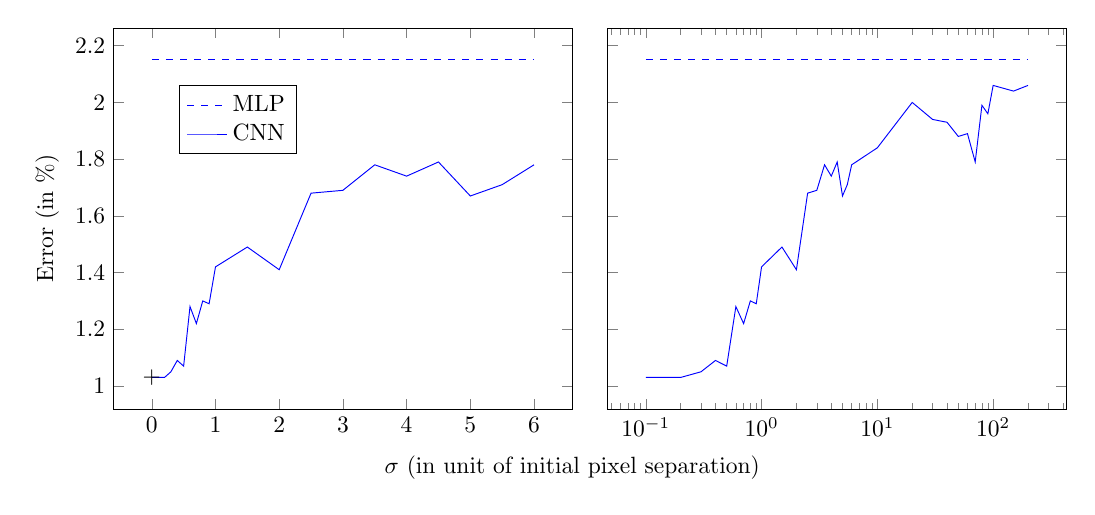
\begin{tikzpicture}[scale=0.85]
    \begin{axis}[xlabel=$\sigma$ (in unit of initial pixel separation), ylabel=Error (in \%),
      legend style={at={(0.4,0.85)}, anchor=north east},
      x label style={at={(axis description cs:1,-0.1)},anchor=north}]

      \addplot[color=blue,dashed,mark=.] coordinates {
        (0.0, 2.15) (6.0, 2.15)
      };

      \addplot[color=blue,mark=.] coordinates {
      (0.0, 1.03)
      (0.1, 1.03)
      (0.2, 1.03)
      (0.3, 1.05)
      (0.4, 1.09)
      (0.5, 1.07)
      (0.6, 1.28)
      (0.7, 1.22)
      (0.8, 1.30)
      (0.9, 1.29)
      (1.0, 1.42)
      (1.5, 1.49)
      (2.0, 1.41)
      (2.5, 1.68)
      (3.0, 1.69)
      (3.5, 1.78)
      (4.0, 1.74)
      (4.5, 1.79)
      (5.0, 1.67)
      (5.5, 1.71)
      (6.0, 1.78)
      };

      \node at (0.0, 1.03) {+};
      %\node at (0.0, 1.10) {\scriptsize{CNN}};

      \legend{MLP, CNN}
    \end{axis}

    \begin{scope}[xshift = 210pt]
      \begin{semilogxaxis}[yticklabels={,,}]

        %\node at (0.1, 1.49) {+};

        \addplot[color=blue,mark=.] coordinates {
        (0.0, 1.03)
        (0.1, 1.03)
        (0.2, 1.03)
        (0.3, 1.05)
        (0.4, 1.09)
        (0.5, 1.07)
        (0.6, 1.28)
        (0.7, 1.22)
        (0.8, 1.30)
        (0.9, 1.29)
        (1.0, 1.42)
        (1.5, 1.49)
        (2.0, 1.41)
        (2.5, 1.68)
        (3.0, 1.69)
        (3.5, 1.78)
        (4.0, 1.74)
        (4.5, 1.79)
        (5.0, 1.67)
        (5.5, 1.71)
        (6.0, 1.78)
        (10.0, 1.84)
        (20.0, 2.00)
        (30.0, 1.94)
        (40.0, 1.93)
        (50.0, 1.88)
        (60.0, 1.89)
        (70.0, 1.79)
        %(75.0, 1.91)
        (80.0, 1.99)
        (90.0, 1.96)
        (100.0, 2.06)
        (150.0, 2.04)
        (200.0, 2.06)
        };

        \addplot[color=blue,dashed,mark=.] coordinates { 
        (0.0, 2.15)
        (0.1, 2.15)
        (200.0, 2.15)
        };

      \end{semilogxaxis}
    \end{scope}

  \end{tikzpicture}
  \caption{Error in function of the standard deviation $\sigma$, for generalized CNNs and an MLP, each with $500$ weights.}
  \label{fig:expres}
\end{figure}